\chapter{Overview of currently used techniques}
This chapter will introduce the techniques used to simulate destructible environments. Historical development of those techniques and a few game engines with unique approaches. In this chapter we will use word object as a reference to buildings, crates, doors, etc., excluding terrain, skyboxes, other players and non-playable characters.

\section{Object replacement or removal}
This was the first method used to simulate destructible environment in a computer game. Mostly because it's simple and undemanding. In spite of it's simplicity it can still produce a very desirable results. In fact it is still most widely used approach to destructible environment in computer games.

The first 2D games featuring destructible environment are arcade games like \emph{Space Invaders (1978)} \cite{invaders} where the environment is represented by a cells in a grid. After first few hits the texture of the cell is replaced by another one and the finally completely removed. The next environment destruction step in 2D games came with games like \emph{Scorched Earth (1991)} \cite{scorched} and \emph{Worms (1995)} \cite{worms}. Collision and removal of terrain in this games is based on individual pixels which creates more realistic visual effect and better gameplay.

Most common implementation of destructible objects in 3D games have not changed much over the years. Every object that the player is supposed to be able to modify has a bunch of other models prepared. Based on how much damage is applied, the models are swapped and eventually removed completely. To make the removal look natural it is usually accompanied by animations, debris and dust generation. This downfall of this method is the necessity to replace the whole in-game object and to make the game look realistic there has to be large number of options for every stage of destruction.

\begin{figure}[h]
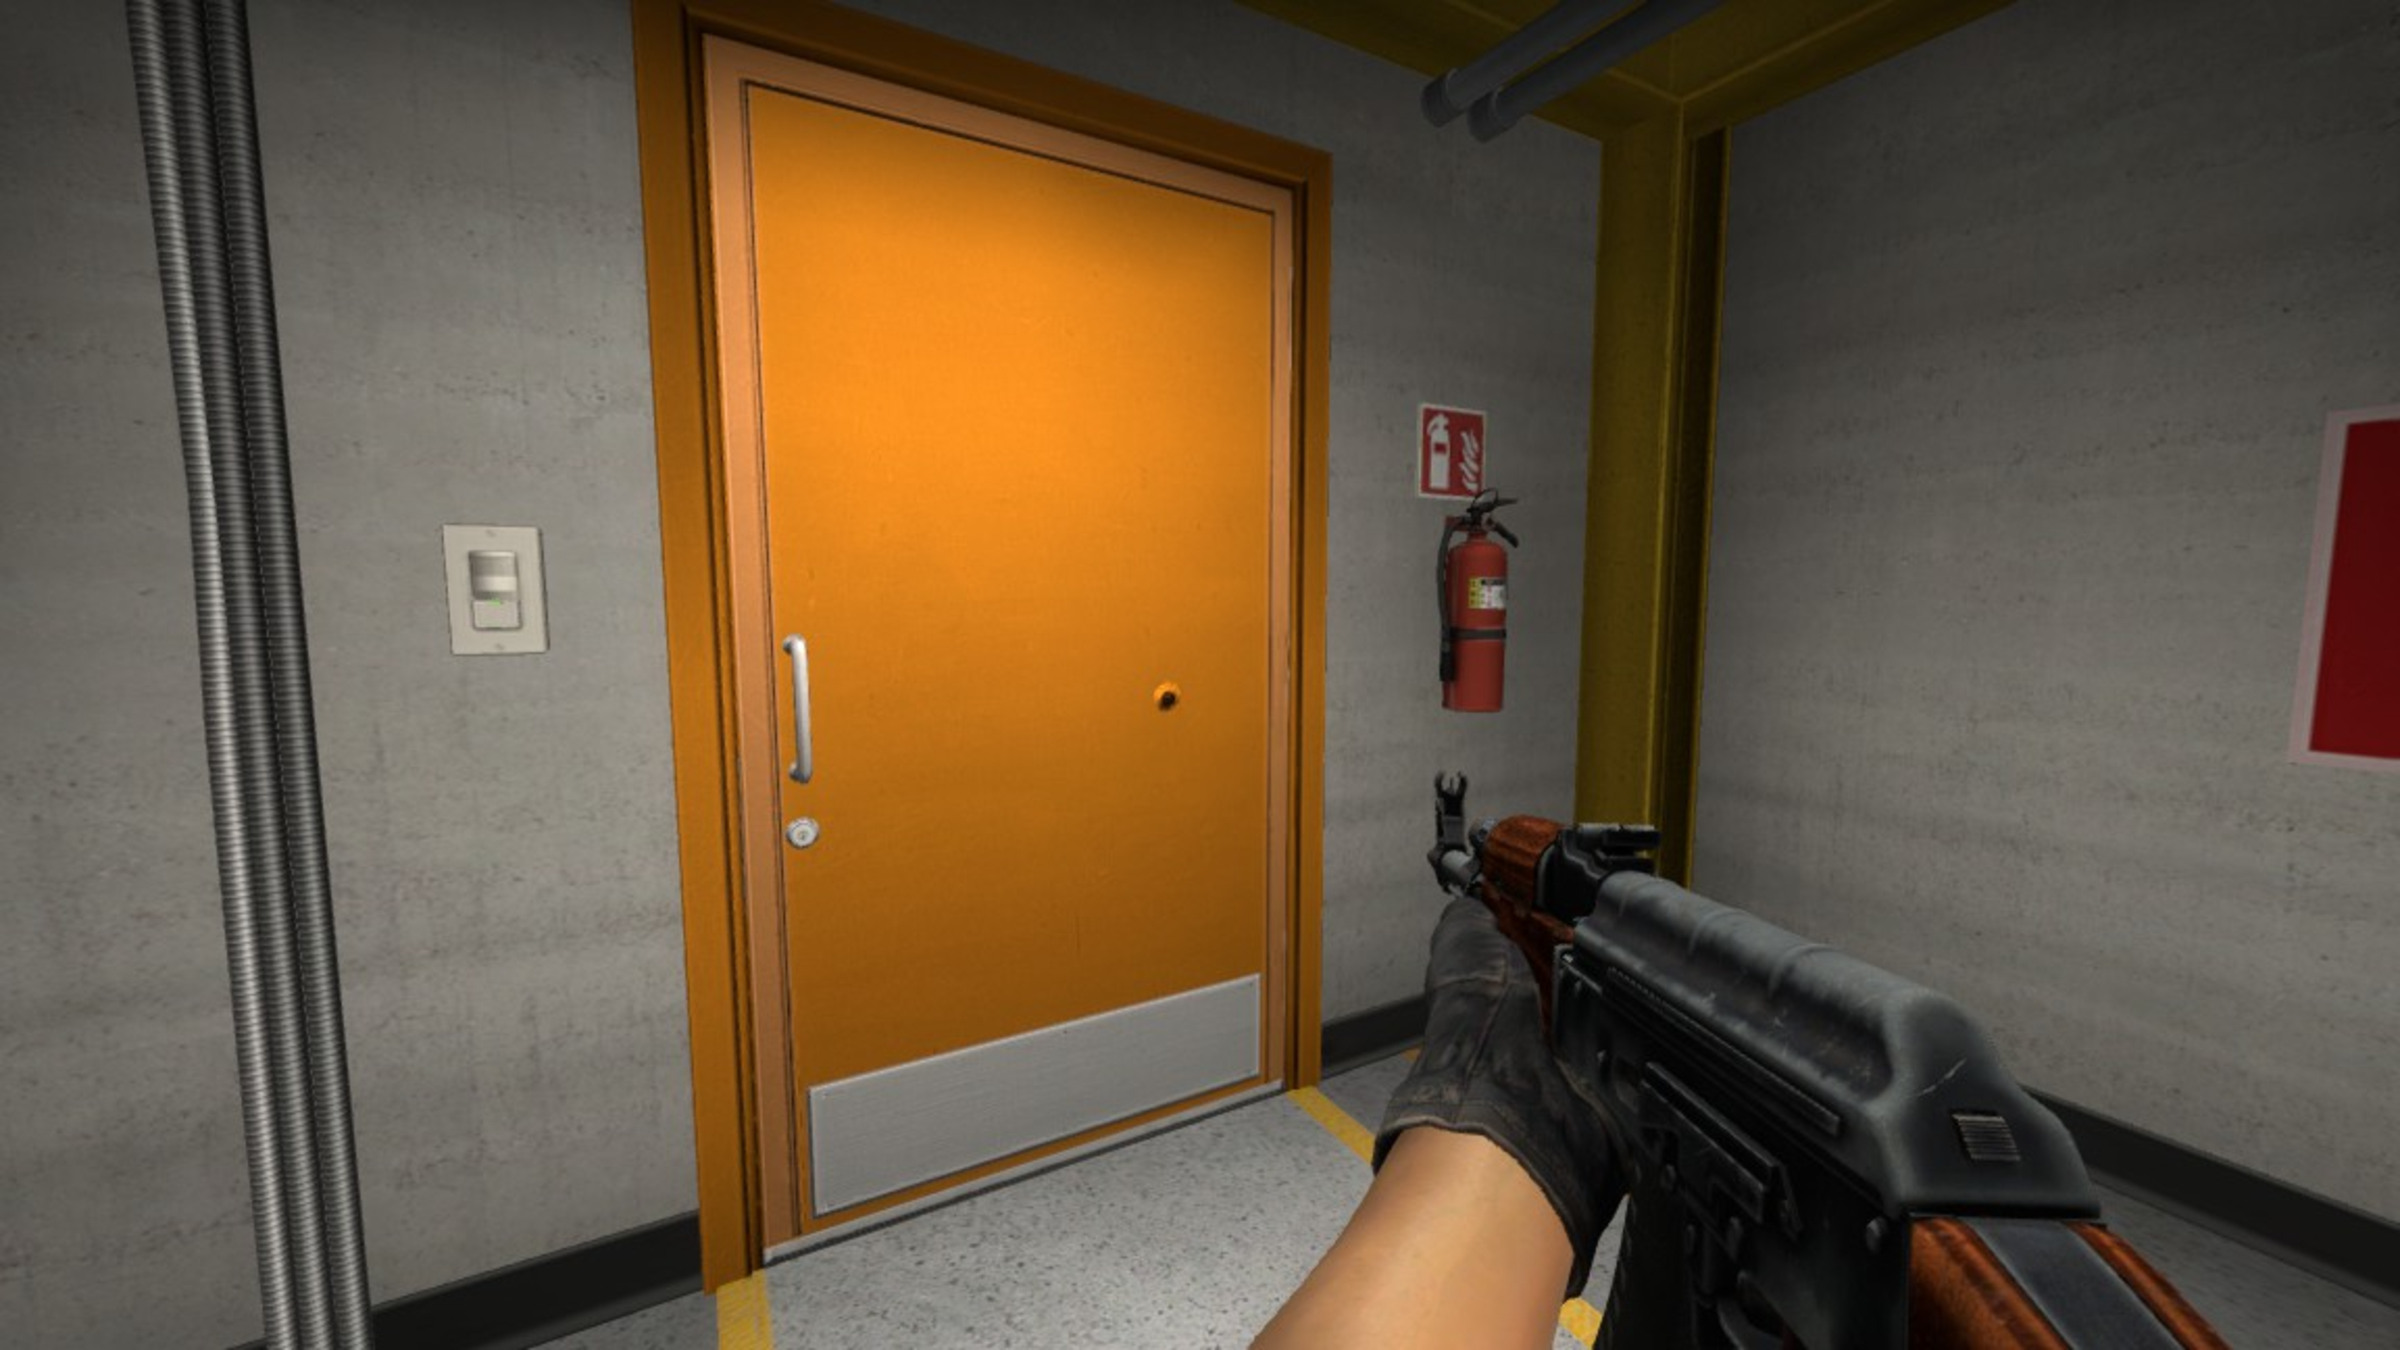
\includegraphics[width=8cm]{img/door1}
\end{figure}

\section{Geo-Mod}
\emph{Geo-Mod} \cite{geomod} or \emph{Geometry Modification Technology} is an engine developed for the \emph{Red Faction (2001)} \cite{redfaction} video game. It allows players to modify and make holes in the terrain using then unique solution of creating objects representing an empty space. Even though the engine doesn't work well with the buildings and other objects, it represents the first major attempt to create fully destructible 3D environment in real time constraints.

\section{Geo-Mod 2}
Unlike it's predecessor \emph{Geo-Mod 2} \cite{geomod}\footnote{Geo-Mod 2.0 presentation video https://www.youtube.com/watch?v=lICurOVsNv0} does not feature destructible terrain, instead it uses physics simulation on specially prepared objects. A set of objects is used as a ragdoll for stress-based simulation model. This limits the engine in the scale of the game world and mutual proximity of destructible objects.

\section{Frostbite}
\emph{Frostbite} \cite{frostbite} engine and mainly it's component \emph{Destruction} \cite{destruction} is currently one of the most popular destruction engines out there. It supports destruction on different scales, the dynamic micro-destruction on the surface and the large scale predetermined destruction on whole buildings. The buildings are created from smaller parts linked together. Each part can disappear on it's own and when there is not much left the whole building goes away under cover of animation. 
It doesn't use inner body stress or basically any physics while doing this simulation.

\section{Precomputed fractures}


\section{Material Point method}

\section{Voronoi fracture}

\section{Finite Element Method}
Finite Element Method(FEM) is a means to simulate behavior of complex objects and systems.  It uses a large number of finite volumes(cells), interconnected or not, to simulate the reaction of material to inner and outside forces. Each cell computes it's own physics states like stress or temperature and propagates the results to neighboring cells. This allow for simulation of fluid dynamics, brittle fractures \cite{brittlefracture}, ductility \cite{ductilefracture}, elasticity, heat transfer and other physical properties. It is very useful in engineering and in modeling and rendering scenes for computer generated images but FEM requires a lot of computational resources and therefore until recently it wasn't possible to implement it in real-time environment of computer game. Now with better hardware and optimized algorithms specially developed for real-time animation, like the one O'Brien \cite{femingames} describes this method is making it's way into modern games.




